\chapter{Ranking}

\section{Classificazione multiclasse e multilabel}
Nella classificazione multi classe ogni esempio ha esattamente una label che sono pertanto mutualmente esclusive.
Nella classificazione multi label ogni esempio ha zero o pi\`u labels, dette anche annotazioni \ref{fig:chapter07-00}. 
Per svolgere una classficazione multi label basterebbe fare training su un modello per ogni label e applicarli a ogni nuovo esempio, ma ci sono altri metodi pi\`u sofisticati ed efficaci come il joint learning.

\begin{figure}
	\centering
	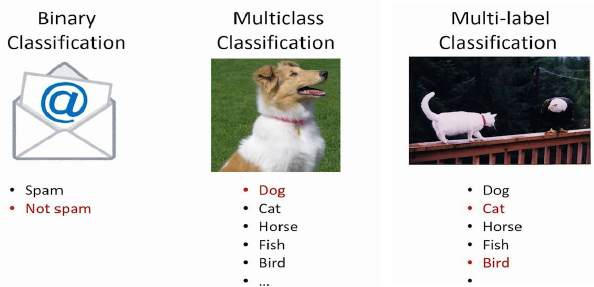
\includegraphics[width=0.6\linewidth]{imgs/chapter7/img0}
	\caption{Riassunto}
	\label{fig:chapter07-00}
\end{figure}

\section{Problema del ranking}
I dati di training sono divisi in $K$ categorie ognuna delle quali corrispondente a un ranking.
Si deve insegnare a un modello che quando riceve un insieme di esempi li fitti nel ranking corretto o ritorni un ordinamento per questo nuovo esempio.

	\subsection{Preference function}
	La preference function o binary classifier \`e un'implementazione di ranking.
	Data una query $q$ e due campioni $x_i$ e $x_j$ il classificatore predice se $x_i$ deve essere preferito a $x_j$ rispetto alla query $q$.
	Il classificatore prende pertanto due campioni e d\`a in output $1$ se il primo \`e pi\`u alto o $-1$ se \`e pi\`u basso.
	In questo modo si ottiene una funzione di ordinamento atomica che si pu\`o estendere a diversi esempi.

		\subsubsection{Perceptron}
		Per implementare questo algoritmo si pu\`o utilizzare il perceptron creando il vettore delle feature combinate dei due esempi:
		$$f'_i = a_i -b_i$$
		$$f'_i = \begin{cases}1\ if\ a_i > b_i\\0\ altrimenti\end{cases}$$
		Questa funzione viene sviluppata in maniera dipendente dall'applicazione.
		Un modo per computare il ranking numerico per i campioni pu\`o essere risolto utilizzando la preference function sommando i valori di ritorno di ogni classificatore e ottenendo uno score per ognuno di essi.

\section{Utilizzo del ranking e della preference function}
Con gli algoritmi visti precedentemente si potrebbe pesare il ranking di un esempio utilizzando la distanza dagli altri.
Si possono usare diversi metodi di distanza dati che sono consistenti.
La distanza a tempo di testing \`e calcolata come la confidenza della predizione del perceptron e d\`a un ordinamento degli esempi.
In questo modo si ottiene una forma di ranking pi\`u precisa rispetto a quella vista prima.
Per un algoritmo di ranking sofisticato si devono incorporare queste osservazioni a tempo di training: se un problema ritorna un'alta differenza in preferenza tra due esempi dovrebbe avere un peso pi\`u alto.

\section{Naive Ranking}

	\subsection{Training}
	\begin{algorithm}[H]
\DontPrintSemicolon
\SetKwComment{comment}{$\%$}{}
\SetKw{Int}{int}
\SetKw{To}{to}
\SetKw{IsNot}{is not}
\SetKw{Is}{is}
\SetKw{Not}{not}
\SetKw{Return}{return}
\SetKw{And}{and}
\SetKw{Require}{return}
\SetKwData{Item}{item}
\SetKwFunction{Min}{min}
\SetKwFunction{BinaryTrain}{BinaryTrain}
\SetKwFunction{NRT}{NaiveRankTrain}

\caption{\protect\NRT{RankingData, \protect\BinaryTrain}}
$D = []$\;
\For{$n = 1$ \To $N$}{
	\For{all $i,j = 1$ to $M$ \And $i\neq j$}{
		\If{$i$ \Is prefered to $j$ on query $n$}{
			$D = D\oplus (x_{nij},-1)$
		}
	}
}
\Return \BinaryTrain{D}
\end{algorithm}


	\subsection{Testing}
	\begin{algorithm}[H]
\DontPrintSemicolon
\SetKwComment{comment}{$\%$}{}
\SetKw{Int}{int}
\SetKw{To}{to}
\SetKw{IsNot}{is not}
\SetKw{Is}{is}
\SetKw{Not}{not}
\SetKw{Return}{return}
\SetKw{And}{and}
\SetKw{Require}{return}
\SetKwData{Item}{item}
\SetKwFunction{Min}{min}
\SetKwFunction{BinaryTrain}{BinaryTrain}
\SetKwFunction{NRT}{NaiveRankTest}
\SetKwFunction{Argsort}{ArgSort}

\caption{\protect\NRT{$f$, $\hat{x}$}}
$score = \langle 0,\dots, 0\rangle$\;
\For{all $i,j = 1$ \To $M$ \And $i\neq j$}{
	$y = f(\hat{x}_{ij})$\;
	$score_i = score_i + y$\;
	$score_j = score_j - y$\;
}
\Return \Argsort{score}
\end{algorithm}


\section{Bipartite ranking}
Gli algoritmi di ranking bipartito risolvono problemi in cui si tenta di predire una risposta binaria, per esempio: "Questo documento \`e rilevante alla ricerca?".
L'obiettivo \`e di assicurare che tutti gli esempi rilevanti si trovano prima di quelli irrilevanti.
Non si trova un ordinamento tra esempi rilevanti.


\section{Ordinamento e $\mathbf{\omega}$-ranking}
Nonostante la veloce soluzione dell'ordinamento con la funzione di preference, si pu\`o utilizzarla come funzione di sorting.
Si definisce un ranking come una funzione $\sigma$ che mappa gli oggetti alla posizione nella lista di ranking desiderata $(1,\dots,M)$.
Se $\sigma_u < \sigma_v$ allora $u$ \`e preferito a $v$.
Dati i dati con ranking osservati $\sigma$ l'obiettivo \`e di imparare a predire i ranking per nuovi oggetti $\sigma^*$.
Si definisce $\sum_M$ l'insieme di tutte le funzioni di ranking su $M$.
Si vuole modellare il fatto che uno sbaglio su alcune coppie \`e peggiore rispetto ad altre, pertanto si implementa una nuova funzione di errore per questo scopo.
Si definisce una funzione di costo $\omega$ dove $\omega(i,j)$ \`e il costo di mettere qualcosa nella posizione $j$ quando dovrebbe essere in $i$.
Tale funzione deve essere:
\begin{multicols}{2}
	\begin{itemize}
		\item Simmetrica: $w(i,j) = w(j,i)$.
		\item Monotona: $i<j<k\lor i>j>k \Rightarrow \omega(i,j) \le \omega(i,k)$.
		\item Soddisfi la disuguaglianza triangolare: $\omega(i,j)+\omega(j,k) \ge \omega(i,k)$.
	\end{itemize}
\end{multicols}
Un esempio, tenendo validi le prime $K$ predizioni, potrebbe essere:
$$\omega(i,j) = \begin{cases}1\ if\ min\{i,j\} \le K \land i\neq j\\ 0\ altrimenti\end{cases}$$
Questa viene detta task di $\omega$ ranking.
Dati:
\begin{itemize}
	\item Uno spazio di input $\mathcal{X}$.
	\item Una distribuzione sconosciuta $\mathcal{D}$ su $\mathcal{X}\times\sum_M$.
	\item Un training set $D$ campionato da $\mathcal{D}$.
\end{itemize}
Si deve computare una funzione $f:\mathcal{X}\rightarrow\sum_M$ che minimizzi:
$$\mathbb{E}_{(\mathcal{X},\sigma)\sim\mathcal{D}}\biggl[\sum\limits_{u\neq v}[\sigma_u < \sigma_v][\hat{\sigma}_v < \hat{\sigma}_u]\omega(\sigma_u,\sigma_v)\biggr]$$
Dove $\hat{\sigma} = f(x)$. I passaggi definiti dentro le parentesi quadre possono essere viste come un booleano. Ad esempio se ho che $[\sigma_u < \sigma_v]$
è verificato e anche la predizione $[\hat{\sigma}_v < \hat{\sigma}_u]$ è verificata allora ho che la funzione di costo $\omega(\sigma_u,\sigma_v)$ viene sommata alla loss function. 
Questo perché ho trovato un caso in cui la predizione è diversa dalla ground truth.

	\subsection{Testing}
	A tempo di testing invece di predirre score e poi ordinare la lista come negli algoritmi prima si utilizza un algoritmo di ordinamento utilizzando la funzione imparata come funzione di ordinamento.
	In pratica ad ogni passo si sceglie un pivot $p$ e ogni oggetto $u$ viene confrontato con $p$ utilizzando la funzione imparata e ordinato a destra o a sinistra.
	La differenza \`e che qua la funzione di comparazione \`e probabilistica.

	\subsection{Implementazione}

		\subsubsection{Algoritmo di train}
		
\begin{algorithm}[H]
\DontPrintSemicolon
\SetKwComment{comment}{$\%$}{}
\SetKw{Int}{int}
\SetKw{To}{to}
\SetKw{IsNot}{is not}
\SetKw{Is}{is}
\SetKw{Not}{not}
\SetKw{Return}{return}
\SetKw{And}{and}
\SetKw{Require}{return}
\SetKwData{Item}{item}
\SetKwFunction{Min}{min}
\SetKwFunction{BinaryTrain}{BinaryTrain}
\SetKwFunction{NRT}{OmegaRankTest}
\SetKwFunction{Argsort}{ArgSort}
\SetKwFunction{Sign}{Sign}

\caption{\protect\NRT{$D^{rank}$, $\omega$, \protect\BinaryTrain}}
$D^{bin} = []$
\For{all $(x,\sigma)\in D^{rank}$}{
	\For{all $u\neq v$}{
		$y =$ \Sign{$\sigma^v$, $\sigma_u$}\;
		$w = w(\sigma_u, \sigma_v)$\;
		$D^{bin} = D^{bin}\oplus(y, w, x_{uv})$\;
	}
}
\Return \BinaryTrain{$D^{bin}$}
\end{algorithm}


		\subsubsection{Algoritmo di test}
		A tempo di test, al posto di prevedere gli score e poi ordinare la lista, utilizziamo l'algoritmo quicksort, utilizzando la funzione imparata come funzione di comparazione. Nella pratica ad ogni passo un pivot $p$ \`e scelto, ogni oggetto $u$ \`e confrontato con $p$ utilizzando la funzione e ordinato a destra o sinistra. La differenza tra questo algoritmo e quicksort \`e che la funzione di comparazione \`e probabilistica.
		\begin{algorithm}[H]
\DontPrintSemicolon
\SetKwComment{comment}{$\%$}{}
\SetKw{Int}{int}
\SetKw{To}{to}
\SetKw{IsNot}{is not}
\SetKw{Is}{is}
\SetKw{Not}{not}
\SetKw{Return}{return}
\SetKw{And}{and}
\SetKw{Or}{or}
\SetKw{Require}{return}
\SetKwData{Item}{item}
\SetKwFunction{Min}{min}
\SetKwFunction{BinaryTrain}{BinaryTrain}
\SetKwFunction{NRT}{OmegaRankTest}
\SetKwFunction{Argsort}{ArgSort}

\caption{\protect\NRT{$f$, $\hat{x}$, obj}}
\If{obj contains $0$ \Or $1$ elements}{
	\Return obj
}
\Else{
	$p = $randomply chosen object in obj\;
	$left = []$\;
	$right = []$\;
	\For{all $u\in obj\backslash\{p\}$}{
		$\hat{y} = f(x_{up})$\;
		\If{uniform random variable $< \hat{y}$}{
			$left = left\oplus u$\;
		}
		\Else{
			$right = right\oplus u$\;
		}
	}
	$left = $\NRT{$f$, $\hat{x}$, $left$}\;
	$right = $\NRT{$f$, $\hat{x}$, $right$}\;
	\Return $left\oplus\langle p \rangle\oplus right$\;
}


\end{algorithm}

\section{Riassunto}

Per l'implementazione più semplice di un modello di classificazione si può utilizzare un classificatore lineare: questo può essere sufficiente per un problema di classificazione bipartita.
Un modello di classificazione più sofisticato può essere sviluppato introducendo una funzione di costo e ideando un modello di test basato su una versione probabilistica di quicksort, che a differenza di prima prende in considerazione la confidenza $\hat{y}$ del modello per ordinare gli esempi.
